% Spikes n 1_(0,1/n) lose their mass; sqrt(n) 1_(0,1/n) are uniformly integrable. Generated by a short script.
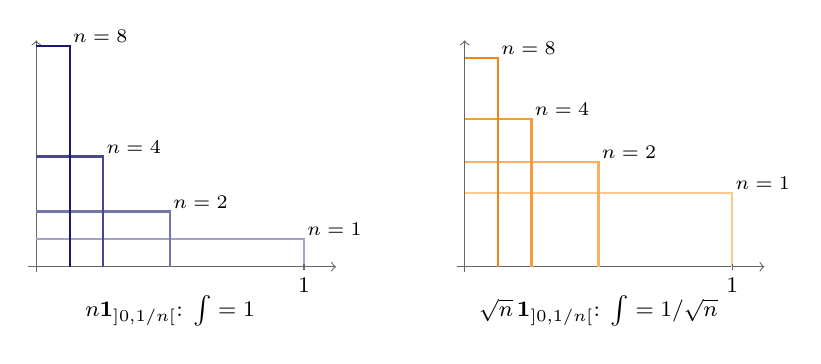
\begin{tikzpicture}[xscale=3.4,yscale=1.25]
\draw[->,black!60] (-0.03,0) -- (1.12,0);
\draw[->,black!60] (0,-0.05) -- (0,2.3);
\draw[MidnightBlue!40,thick] (0,0.280) -- (1.000,0.280) -- (1.000,0);
\node[font=\scriptsize,above right,inner sep=1pt] at (1.000,0.280) {$n=1$};
\draw[MidnightBlue!60,thick] (0,0.560) -- (0.500,0.560) -- (0.500,0);
\node[font=\scriptsize,above right,inner sep=1pt] at (0.500,0.560) {$n=2$};
\draw[MidnightBlue!80,thick] (0,1.120) -- (0.250,1.120) -- (0.250,0);
\node[font=\scriptsize,above right,inner sep=1pt] at (0.250,1.120) {$n=4$};
\draw[MidnightBlue!100,thick] (0,2.240) -- (0.125,2.240) -- (0.125,0);
\node[font=\scriptsize,above right,inner sep=1pt] at (0.125,2.240) {$n=8$};
\node[font=\footnotesize,below] at (1,-0.02) {$1$};
\draw[black!60] (1,0.03) -- (1,-0.03);
\node[font=\footnotesize] at (0.5,-0.45) {$n\mathbf 1_{]0,1/n[}$: $\int=1$};
\draw[->,black!60] (1.57,0) -- (2.72,0);
\draw[->,black!60] (1.6,-0.05) -- (1.6,2.3);
\draw[BurntOrange!40,thick] (1.6,0.750) -- (2.600,0.750) -- (2.600,0);
\node[font=\scriptsize,above right,inner sep=1pt] at (2.600,0.750) {$n=1$};
\draw[BurntOrange!60,thick] (1.6,1.061) -- (2.100,1.061) -- (2.100,0);
\node[font=\scriptsize,above right,inner sep=1pt] at (2.100,1.061) {$n=2$};
\draw[BurntOrange!80,thick] (1.6,1.500) -- (1.850,1.500) -- (1.850,0);
\node[font=\scriptsize,above right,inner sep=1pt] at (1.850,1.500) {$n=4$};
\draw[BurntOrange!100,thick] (1.6,2.121) -- (1.725,2.121) -- (1.725,0);
\node[font=\scriptsize,above right,inner sep=1pt] at (1.725,2.121) {$n=8$};
\node[font=\footnotesize,below] at (2.6,-0.02) {$1$};
\draw[black!60] (2.6,0.03) -- (2.6,-0.03);
\node[font=\footnotesize] at (2.1,-0.45) {$\sqrt n\,\mathbf 1_{]0,1/n[}$: $\int=1/\sqrt n$};
\end{tikzpicture}
